\section{FIR - Finite Impulse Response}\label{sec:fir}
Formålet med FIR filteret er at udregne filter koefficienterne, $b_{i}$, der bruges til at approksimere størrelsen af frekvens responset af FIR filteret $H(z)$.
Forholdet mellem input og output i er FIR filter er givet ved ligning \ref{fir_ligning},
\begin {equation} 
y(n)=\sum\limits_{i=0}^{K}b_{i}x(n-i) \label{fir_ligning}
\end {equation}
hvor $b_{i}$ repræsenterer filterets koefficienter og $K+1$ er filterets længde.
\\
Derefter z-transformeres ligning \ref{fir_ligning}. For at opskrive FIR filterets overføringsfunktion, faktoriseres $X(z)$ ud på højre side af den z-transformerede ligning \ref{fir_ligning} og derefter dividere igennem med $X(z)$ fås ligning \ref{fir_transfer}.

\begin {equation}
H(z)=\frac{Y(z)}{X(z)}=b_{0}+b_{1}z^{-1}+...+b_{K}^{-1} \label{fir_transfer}
\end {equation}

Input og output signalet er givet ved foldning og er opskrevet i ligning,
\begin {equation} 
\sum\limits_{i=0}^{N-1} h(k)x(n-k) 
\end {equation}
hvor $h(k)$ er impulsresponset modsat IIR filterne har en endelig længde, $N$, antal værdier. FIR filterets impulsrespons er et sæt af filter koefficienter. Sendes en impuls ind i filteret bestående af et $"1"$ efterfulgt af mange $"0"$er, bliver filterets output det sæt af koefficienter $"1"$-samplen kører igennem. 


FIR filterets overføringsfunktion er givet ved ligning \ref{FIR_transfer}

\begin {equation}
H(z)=\sum\limits_{k=0}^{N-1}h(k)z^{-1} \label{FIR_transfer}
\end {equation}
\section{Design metoder} \label{sec:fir_design}
Herunder redegøres der for 3 forskellíge design metoder, til beregning af filter koefficienter.
Frekvenssamplingsmetoden vil være mere dybdegående end de to andre, da det er den metode der vil blive implementeret.
\subsection{Frekvenssampling}
Ved frekvenssampling approksimeres det ønskede frekvensrespons ved, at sample det $N$ antal gange, med samme interval imellem samplingspunkterne. Der kan derved opnås et interpolateret frekvens respons.
Pointen med frekvenssampling er at filterkoefficienter kan beregnes udfra specificerede størrelser i forhold det ønskede filter respons uniformt i frekvensdomænet.

Filterkoefficienterne kan beregnes udfra definitionen af den inverse DFT (IDFT):

\begin {equation}
h(n)=\frac{1}{N}\sum_{k=0}^{N-1}H_{d}(k)W_{N}^{-kn} ,\hspace{1cm}\text{for}\hspace{1cm} n = 0, 1,\text{ ... }, N-1 \label{fir_filterkoefficienter}
\end {equation}
hvor
\begin {equation}
W_{N}=e^{j\frac{2\pi}{N}} \hspace{1cm}\text{og} \hspace{1cm} H_{d}(k)=h(e^{j\Omega_{k}}) \nonumber
\end {equation}
Det antages lineær fase og at antallet af samplingspunkt er $N=2M+1$.


\begin{figure}[h]
\centering
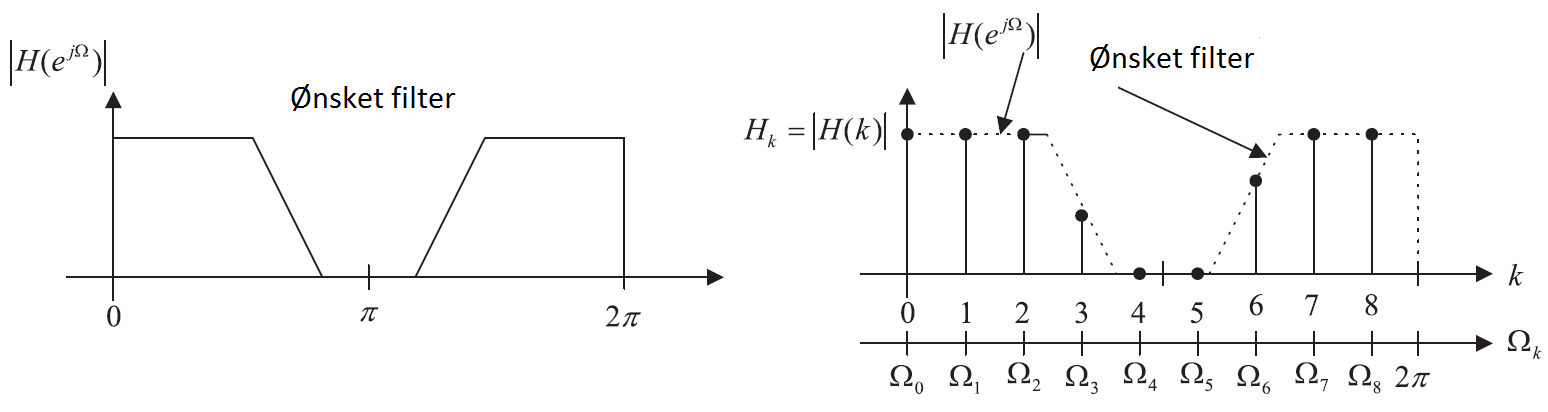
\includegraphics[width=.90\textwidth]{billeder/fir_frekvenssampling.png}\label{fig:fir_frekvenssampling}
\caption{Ønskede filterrespons og samplede filterrespons.}
\end{figure}
\FloatBlock
Ligning \ref{fir_filterkoefficienter} kan simplificeres til,
\begin {equation}
h(n)=\frac{1}{2M+1}\left[ H_{0}+2\sum_{k=1}^{M} \left( \frac{2\pi k(n-M)}{2M+1} \right) \right] \hspace{1cm} \text{for} \hspace{1 cm} n=0,1,\text{ ... },2M
\end {equation}

hvor $h(k)$ for $k=0,1,\text{ ... },2M$, repræsenterer filterkoefficienternes størrelser, der bruges til at specificere det ønskede filterrespons med samplingslængden $\Omega_{k}=\frac{2\pi k}{(2M+1)}$.



\subsection{Windowsmetoden}

\subsection{Equiriple}